
\section{Moment of Inertia}

\makelabheader %(Space for student name, etc., defined in master.tex or labmanual_formatting_commands.tex)

\textbf{Objective} 

To investigate Newton's second law of motion for rotating bodies by applying
it to determine the moment of inertia of a disk.

\textbf{Moment of Inertia} 

In this experiment you will determine the moment of inertia of a body by applying
Newton's second law of motion for rotating bodies. The moment of inertia of
a body is a measure of the tendency of the body to resist a change in its state
of rotational motion. When a net external torque, 
$\tau$, acts on a rigid body free
to rotate about some axis, an angular acceleration, 
$\alpha$, is produced that is
proportional to the torque. The proportionality constant is the moment of inertia,
$I$, of the body. This is the rotational analog of Newton's second law of motion. 

The experimental setup is shown in the figure below. The apparatus consists
of a mass, $m$, connected by a string passing over two pulleys to the drum of
a rotator.

\vspace{0.3cm}
{\par\centering 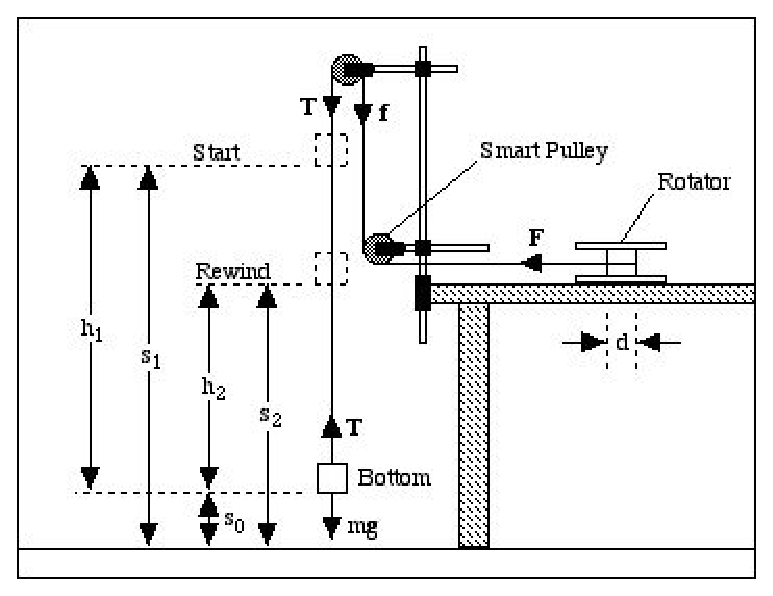
\includegraphics{moment_inertia/moment_inertia_fig1.eps} \par}
\vspace{0.3cm}

\textbf{Apparatus}

\begin{itemize}
\item Rotator
\item Smart pulley
\item Regular pulley
\item Variety of masses
\item String
\item Vernier caliper
\item 2-meter stick
\item \textit{Science Workshop 750 Interface}
\item \textit{DataStudio} software (Atwood's Machine application)
\end{itemize}
\textbf{Activity 1: Prediction for the Moment of Inertia} 

(a) Write the symbolic expression for Newton's second law for rotating bodies
in the space below.
\vspace{10mm}

(b) Write an expression for the net torque on the rotator in terms of the radius
of the rotator drum, $r$, and the magnitude of the net force supplied by the string,
$F$.
\vspace{10mm}

(c) Write an expression for the angular acceleration of the rotator drum in
terms of the radius of the drum, $r$, and the acceleration of the hanging mass,
$a$.
\vspace{10mm}

(d) Notice that the net force on the drum, $F$, is equal to the tension in the
string, $T$, minus the frictional force, $f$. Write an expression for 
$F$ in terms
of $T$ and $f$.
\vspace{10mm}

(e) Apply Newton's second law to the hanging mass to obtain an expression for
the tension, $T$, in terms of $m$, $g$, and $a$.
\vspace{20mm}

(f) The frictional force, $f$, can be determined by application of the principle
of conservation of energy. If the mass, $m$, falls a height, \( h_{1} \), and
then rises a height, \( h_{2} \), on the rewind, the loss in its potential
energy between the two positions is equal to the work done by the frictional
force. Using this, find an expression for $f$ in terms of $m$, $g$, \( h_{1} \),
and \( h_{2} \).
\vspace{20mm}

(g) Combine the equations abov, to get the following expression for the moment
of inertia of the rotator (with or without the disk): 
\[
I=\frac{md^{2}}{4a}\left( g-a-g\frac{h_{1}-h_{2}}{h_{1}+h_{2}}\right) \]
where $d$ is the diameter of the drum of the rotator.
\vspace{40mm}

\textbf{Activity 2: Determining the Moment of Inertia }

(a) Use the vernier caliper to measure the diameter of the drum of the rotator.
Each member of the group should make an independent measurement and record the
average value as $d$. If you have questions about how to read the vernier, consult
your instructor.
\vspace{10mm}

(b) Launch the Atwood's Machine application.

(c) Remove the disk from the rotator and construct a data table below with the
column headings $m$, \( s_{0} \), \( s_{1} \), \( s_{2} \), \( h_{1} \), 
\( h_{2} \),
$a$, and $I$. Don't forget to include appropriate units in the column headings.
\vspace{100mm}

(d) Hang 50 grams on the string and lower the mass slowly until all the string
is unwound from the drum. Measure and record the distance from the bottom of
the mass to the floor as \( s_{0} \).

(e) Rewind the string on the drum until the mass is a few centimeters from the
upper pulley. Measure and record the distance, \( s_{1} \), from the floor
to the mass.

(f) Release the mass, start recording data, and stop it at its highest position
on the rewind. Measure and record the distance, \( s_{2} \), from the floor
to this position of the mass.

(g) The computer will display a graph of the velocity versus time for the fall
of the mass. Fit the data to determine the acceleration and record this value
in your data table.

(h) Repeat steps (d)-(g) two more times for a total of three trials.

(i) Replace the 50 gram mass with a 70 gram mass and repeat steps (d)-(h).

(j) Place the disk on the rotator, construct a new data table, and repeat steps
(d)-(i).
\vspace{100mm}

(k) Calculate and record the moment of inertia for each trial. Show a sample
calculation for one trial in the space below.
\vspace{30mm}

(l) Determine the average value for the moment of inertia of the rotator without
the disk and record his value as \( I_{R} \) below.
\vspace{10mm}

(m) Determine the average value for the moment of inertia of the rotator with
the disk and record this value as \( I_{R+D} \).
\vspace{10mm}

(n) Calculate and record the experimental value for the moment of inertia of
the disk, \( I_{exp}  = I_{R+D} - I_{R} \).
\vspace{10mm}

(o) Calculate the theoretical moment of inertia of the disk, \( I_{th} \),
assuming that it is uniform, and determine the \% difference between \( I_{exp} \)
and \( I_{th} \).
\vspace{40mm}

(p) Does the experimental value for the moment of inertia of the disk agree
with the theoretical value within experimental uncertainties? Do the results
verify Newton's second law of motion for rotating bodies?

